\maketitle

\begin{abstract}
  Current trends suggest building datacenters according to a resource
disaggregated architecture, where resources of the same type are
grouped into a pool and each pool communicates with other pools
using high performance network switches.  This approach transforms
the computer abstraction from one with a fixed set of hardware
resources into one where the set of resources can be changed
on-demand, similar to the virtual resources within a process
abstraction.  We submit that to take full advantage of this paradigm
we have to reconsider the software stack, including the hypervisors,
the operating systems, and eventually the applications themselves.

This paper focuses on the operating system.  We propose that an
operating system running on disaggregated architecture should be
\emph{continuously reconfigurable}, where the hardware resources
available to the operating system are allocated on-demand.  We
present benefits that can be obtained from such a \emph{fluid}
operating system and enumerate challenges and research opportunities.
 \end{abstract}

\section{Introduction}
\label{sec:intro}
Hardware resource disaggregation is a new trend for building
datacenters as it solves several limitations of a traditional monolithic
server architecture~\cite{Intel_RSA, HP_The_Machine, FB_disaggregated_rack,
chung2018towards, katrinis2016rack, asanovic2014firebox,
lim2009disaggregated, shan2018legoos}. A traditional
monolithic architecture consists of a collection of server boxes, with
each box containing a collection of computer resources such as processors,
memory, NICs, and accelerators such as GPUs.
In contrast, in a resource disaggregated datacenter computer resources
are partitioned into \emph{resource blades} connected by high performance
network switches.
Examples of resource blades include processor, memory, and
accelerator blades.
In a disaggregated datacenter there is no longer a
\emph{hard boundary} between different computers.
Instead, hypervisors and operating systems orchestrate
computer abstractions with \emph{soft boundaries}.

\begin{figure}[]
     \centering
     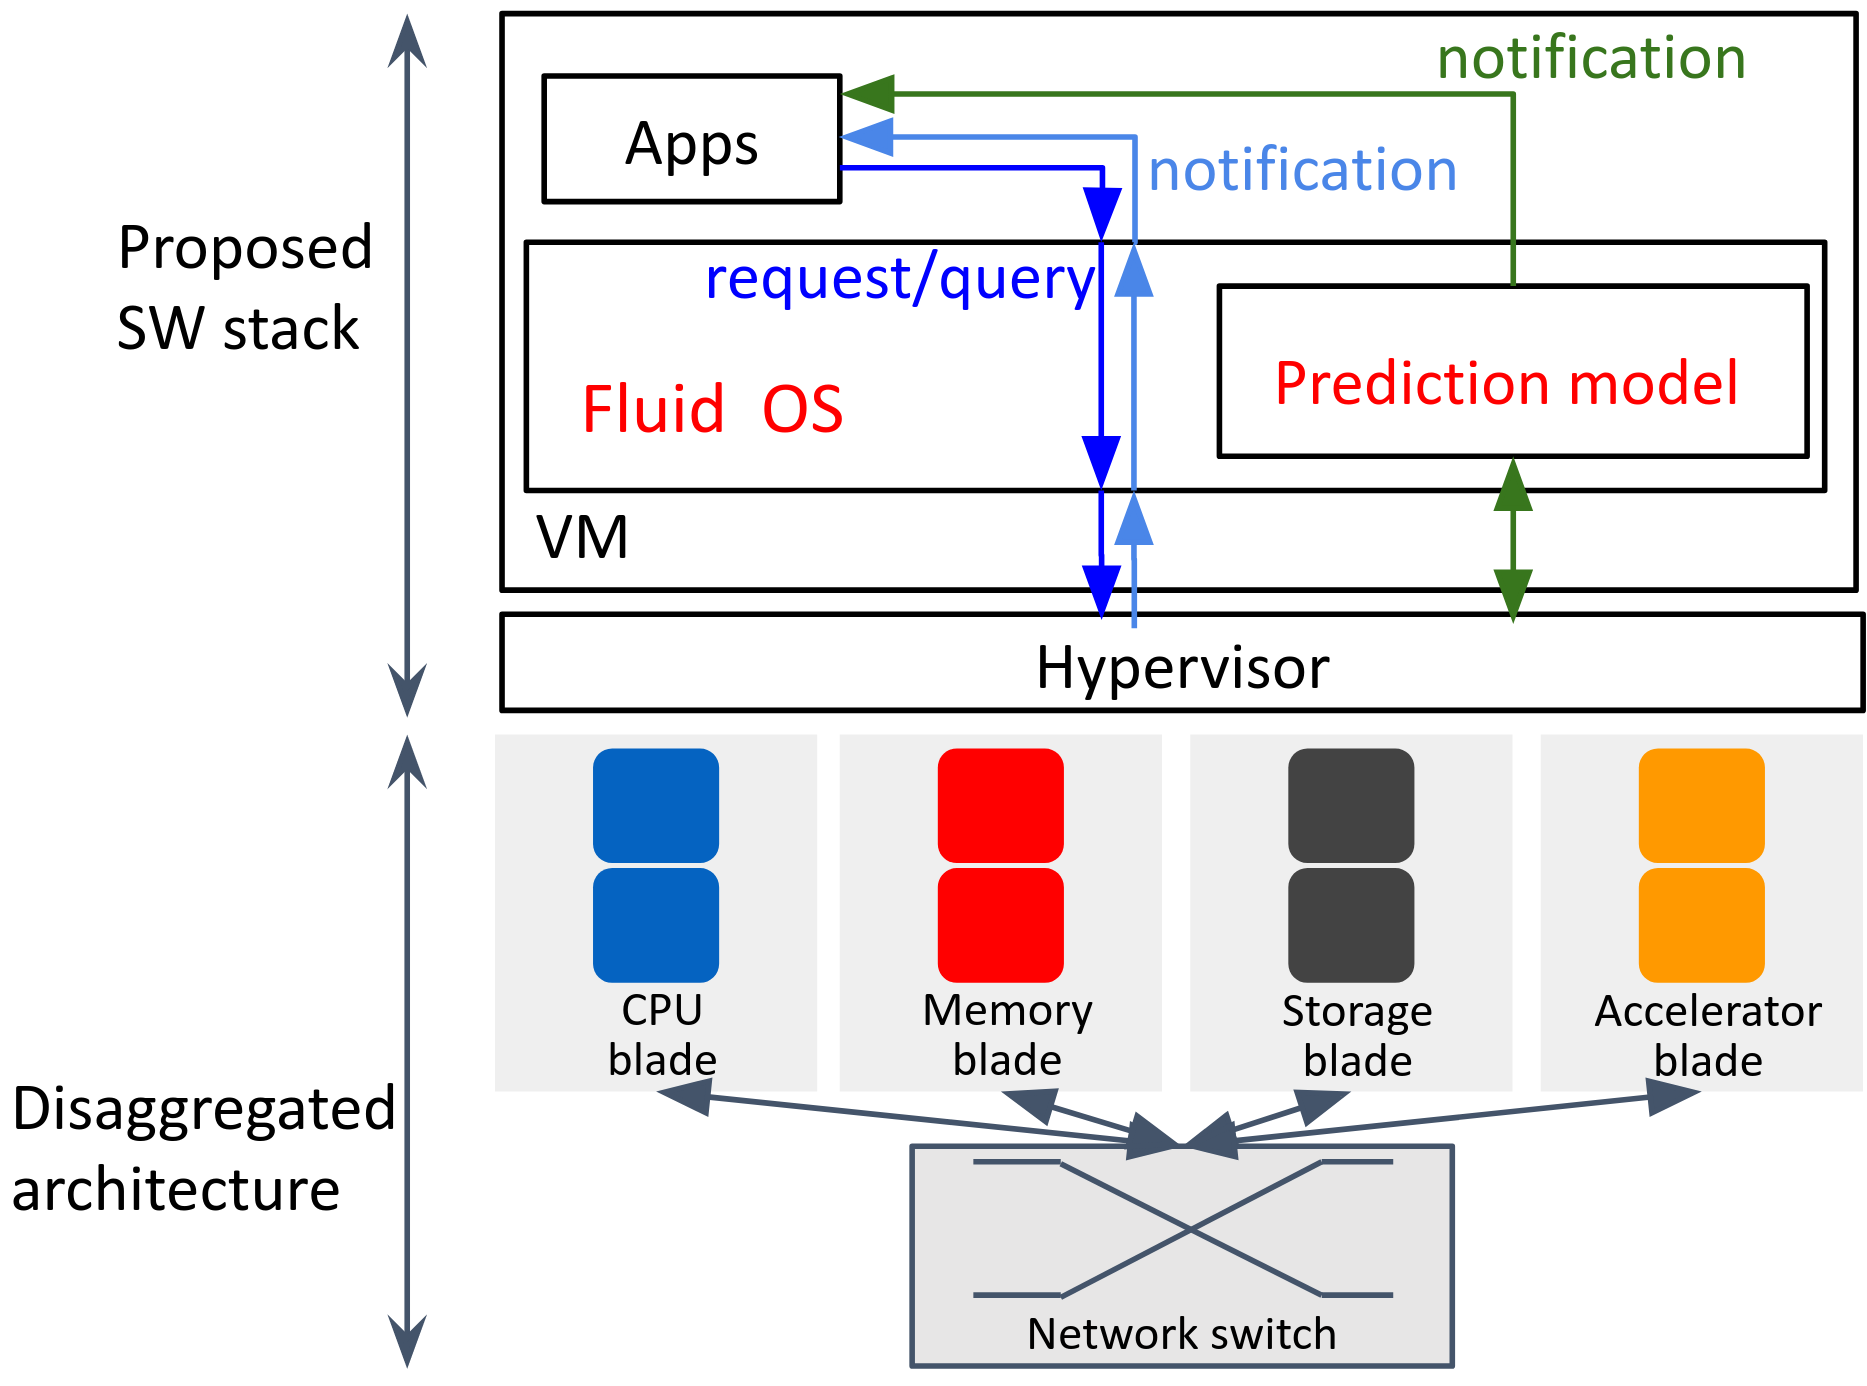
\includegraphics[scale=0.15]{images/architecture.png}
     \caption{Proposed architecture.}
     \label{fig:archi}
\end{figure}


Hardware resource disaggregation further realizes resource
elasticity~\cite{herbst2013elasticity} as computing resources can
be allocated across traditional server boundaries.  In a monolithic
architecture, the resources a virtual machine or container can
allocate are limited by the resources on the hosting physical
machine, while in a disaggregated architecture resource can be
allocated from much larger \emph{resource pools}.  Furthermore, in
a disaggregated architecture, each type of resource can be allocated
independently without considering the amount or availability of
other types of resources.  Because resource allocation is essentially
unbounded and independent, disaggregated architectures have the
potential to achieve better utilization than monolithic ones.

\begin{comment}
Take Amazon EC2~\cite{ec2} for example, the computing
resources of each EC2 instance type is pre-defined and fixed (e.g.,
m5.large type consist of 2 vcpu and 8 GIB memory).  This resource
relation constraint can no longer exist in a resource disaggregated
datacenter.
\end{comment}

To take full advantage of the unbounded and independent resource
elasticity, we argue that operating systems running on the resource
disaggregated hardware should be \emph{continuously reconfigurable}.
Here we define a \emph{reconfigurable OS} to be an OS that allows
dynamically changing computing resources. For instance, an OS may
boot with 2 cores and 4 GB memory but it can allocate or deallocate
cores and memory according to its demands. Reconfigurability can
be further extended to storage devices, accelerators, NICs, and so
on.  Moreover, a reconfigurable OS can also support dynamically
allocating different classes of the same computing resource (e.g.,
brawny vs.~wimpy cores for CPU, DRAM, 3D-stacked DRAM, NVM for
memory).

We target public cloud platforms where applications are
running in virtual machines. This assumption is realistic as most
of public cloud providers wrap users' software within virtual
machines. This concept also holds for containerized cloud and
serverless frameworks~\cite{agache2020firecracker}. As depicted in
Figure~\ref{fig:archi}, we assume there is a hypervisor running on
top of the disaggregated hardware and we can rely on it to manage
the underlying disaggregated hardware components. Moreover, this
hypervisor provides a new virtual machine abstraction consisting
of changing hardware resources instead of the fixed set of resources
available in a conventional virtual machine abstraction.

We are prototyping a reconfigurable OS as a guest OS inside
a virtual machine. This allows us to focus on exploring the policies
and mechanisms required for supporting resource reconfiguration
without dealing with subtle hardware settings.
Section~\ref{sec:proposal} presents details about the
proposed architecture.

There are several benefits that can be obtained from
a reconfigurable OS.
\begin{itemize}
\item The approach is optimal for memory-intensive applications as
memory can be allocated as needed.  A reconfigurable OS is also
advantageous to memory-elastic applications~\cite{funaro2020memory}.
\item With the capability of allocating many cores and accelerators
in a single reconfigurable OS, highly compute-intensive
workloads are more easily supported without the need to
explicitly distribute them across multiple machines.
\item The reconfigurable OS better heterogeneous resource usage,
like a workload allocating both brawny and wimpy cores and
different types of memory.
\item As resources can be requested unboundedly and independently,
the proposed architecture enables the Resource-as-a-Service
cloud cost model~\cite{ben2012resource}.
\end{itemize}

\begin{comment}
We elaborate the benefits more in Section~\ref{sec:benefits}. Beyond
that, we hope the support of resource reconfigurability can enable
a new programming paradigm and enlight more research directions.
\end{comment}

The paper is organized as follows.  Section~\ref{sec:background}
provides background and contrast our proposed architecture with
prior work.  We motivate the reconfigurable OS, elaborating on
benefits that can be obtained from the reconfigurable OS in
Section~\ref{sec:reconfig_os}.  We present challenges and research
opportunities in Section~\ref{sec:opportunities}.
Section~\ref{sec:proposal} provides details of our proposed
architecture and in particular the reconfigurable OS.
Section~\ref{sec:conclusion} concludes.
 
\section{Background}
\label{sec:background}
In this section, we review prior work on resource disaggregation,
resource reconfiguration, and OS reconfiguration, and contrast
this with our proposed research.

\subsection{Resource disaggregation}
The concept of resource disaggregation is that instead of building
servers by collecting all required hardware components within a
physical box, different hardware components can be placed into
multiple resource blades, communicating with each other via network
switches (Figure~\ref{fig:archi}). Compared to the traditional
monolithic architecture, a disaggregated architecture provides
better resource utilization, supports hardware upgrade and scaling,
and supports heterogeneous computing.  Commercial systems include
Intel’s Rack Scale Architecture~\cite{Intel_RSA}, HP’s “The
Machine”~\cite{HP_The_Machine}, Facebook’s Disaggregated
Rack~\cite{FB_disaggregated_rack}, and IBM’s Composable
System~\cite{chung2018towards}.  Academic systems include
dRedBox~\cite{katrinis2016rack}, Firebox\cite{asanovic2014firebox},
and disaggregated memory blade~\cite{lim2009disaggregated}.

Several systems have been built that leverage disaggregated memory
to optimize memory-intensive applications, either by remote memory
swapping~\cite{lagar2019software, al2020effectively, gu2017efficient}
or by exposing a remote memory abstraction to
applications~\cite{aguilera2018remote}.  LegoOS~\cite{shan2018legoos}
proposes the \emph{splitkernel} architecture and implements an OS
especially built for disaggregated hardware. Other work
evaluate the networking aspect of achieving resource
disaggregation\cite{abali2015disaggregated, gao2016network}.

While these system explore disaggregate resources, the
operating systems themselves assume that, once booted, the
collection of hardware resources available does not change.
We propose to develop an OS where the set of hardware resources
that it uses is highly fluid and governed by application demand
rather than by hardware limitations.

\subsection{Resource reconfiguration}
In cloud computing, resource \emph{vertical scaling} (aka
\emph{scale-up}) and resource overcommitment raise the need for
resource reconfiguration.  Most prior research focuses on memory
overcommitment and auto-scaling and use memory
ballooning~\cite{waldspurger02} to adjust the memory accessible to
VMs~\cite{salomie2013application, amit2014vswapper, hines2011applications,
agmon2014ginseng, shaikh2015dynamic, molto2013elastic}. These
approaches still have a limited amount of computing resources that
are specified when a VM is booted. We propose to eliminate these
limitations and achieve a high degree of resource reconfiguration.

Similar to our approach are the Resource-as-a-Service cloud
model~\cite{ben2012resource} and nonkernel~\cite{ben2013nonkernel},
which also propose to build an OS that views computing resources
in a fine-grained fashion.  However, these systems target traditional
monolithic servers, while we believe that a disaggregated architecture
would be a better target.


\subsection{Reconfiguration policies}
\cite{sedaghat2013virtual} describes various VM repacking
policies that take either changes in workload or the
total load as input and output a decision on whether to reconfigure,
and if so, the new optimal resource distribution.
For memory-intensive workloads, a study of cloud providers shows that
auto-scaling of the memory resources can be completed by analyzing the
applications' memory miss ratio curve (MRC) and modeling this as a
hyperbola~\cite{novak2020auto}.

Prior research on web applications~\cite{yazdanov2014lightweight}
shows that fine-grained vertical scaling of multi-tiered web
applications can be accomplished through reinforcement learning
models online.  Additionally, with the recent development of machine
learning models, the prediction tasks on the optimal amount of
resources can also be solved by certain supervised deep learning
models.  Since the input is a series of data that is time-correlated,
recurrent neural networks can capture the important features
~\cite{gers1999learning}.

\subsection{OS reconfiguration}
Prior work on OS reconfiguration has focused on updating the
policies or mechanisms of a deployed OS. The main purpose is to
carry out application-specific optimizations, insert third-party
modules, enable dynamic monitoring, or fix bugs on the
fly~\cite{soules2003system, baumann2007reboots, baumann2005providing,
chen2006live, chen2007polus}. Learned OS~\cite{zhang2019learned}
proposes using machine learning to tune and build an OS. We propose
that, in addition to policies and mechanisms, OS reconfiguration
should also include the ability to reconfigure the computing resources
an OS can use.  We are interested in both machine learning and more
traditional heuristics to achieve better resource utilization.
 
\section{Toward a Reconfigurable OS}
\label{sec:reconfig_os}
\subsection{Why a reconfigurable OS?}
Hardware resource disaggregation breaks the conventional image of
what a computer looks like.  Traditionally, an OS is booted with a
fixed set of hardware resources at its disposal, with only limited
and often crude options to change this set while the OS is running.
We propose that to take full advantage of resource disaagregation,
the OS should adopt an on-demand model of resource usage. A
reconfigurable OS can dynamically allocate or de-allocate its
resources as needed.

One approach would be to have reconfigurable OSes provide the
same abstractions to application programmers as traditional
OSes provide, hiding the underlying architecture altogether.
With this approach, application deployment and development
on a disaggregated architecture would be fully transparent.

While attractive, we believe that the OS abstractions offered to
application programmers need to be revisited so applications
can take full advantage of disaggregated resources.
We want to provide new OS abstractions and expose
resource reconfigurability to application programmers.
The applications can then manipulate computing resources to
achieve application-specific optimizations.
We can still support legacy applications, either by providing
a compatibility layer or by running traditional OSes along
side reconfigurable ones.

\subsection{Benefits of a reconfigurable OS}
\label{sec:benefits}
\noindent
\textbf{Higher degree of resource elasticity}.
Disaggregated architecture can achieve resource elasticity beyond
what the traditional monolithic architecture can provide because
the hardware resources are no longer constrained by hard boundaries.
This creates various advantages.

First, this capability allows applications to execute highly parallel
tasks on a single machine (running a reconfigurable OS) without
having to resort to distributed computing frameworks like MapReduce.

Second, a reconfigurable OS supports memory-elastic applications.
As argued in a paper on a memory elasticity
benchmark~\cite{funaro2020memory}, memory-elastic applications have
significant potential that cannot be realized in traditional
architectures.  We believe the reconfigurable OS can fully support
such applications.

Lastly, the reconfigurable OS allows applications to use multiple
accelerators (e.g., GPU, TPU, FPGA, ASIC, etc.) as long as they are
available anywhere in the disaggregated architecture.
In traditional architectures, applications can only use the
accelerators that are locally available.  If a particular accelerator
is needed on demand, the virtual machine would have to be migrated,
potentially losing access to other accelerators.

\noindent
\textbf{New view of computing resources}.
If the resource disaggregated datacenter provides an abundance of
computing resources, a reconfigurable OS enables a new way
of exploiting those resources. We briefly illustrate some of the
potential new uses.

First, a disaggregated datacenter may provide different types of
processor blades such as processors that have both brawny and
wimpy cores~\cite{holzle2010brawny}. Applications running on a
reconfigurable OS can bind to cores that best suit them and adjust
the binding dynamically.

Second, new memory hierarchies can be formed either by speed or
shareability. In terms of speed, a reconfigurable OS can allocate
its memory from different memory technologies (e.g., DRAM, 3D-stacked
DRAM, NVM) that provide different speed versus space trade-offs. As for
shareability, an OS can have some part of memory shared
datacenter-wide, some part shared within a user-defined domain,
and some part for private use. Big-data analytic and serverless
applications usually need to store the short-lived intermediate
data between each computing stage. It can leverage the user-defined
shared memory to store the intermediate data.

Third, different memory components can be configured with different
consistency models. Applications may separate their logic into
control planes, which often require a strong consistency guarantee,
and data planes, which may tolerate relaxed consistency and trade
it for higher performance.

Fourth, applications may be able to use a mixture of non-volatile
and volatile memory, avoiding the need for frequent checkpointing
of data that needs to persist.

 
\section{Research Opportunities}
\label{sec:opportunities}
In this section, we discuss several research opportunities raised by
the fluid OS perspective.

\subsection{Resource reconfiguration mechanisms}  The key to
designing an effective fluid OS is to support frequent or even
continuous resource reconfigurations.
The response time of each reconfiguration
should be especially considered.  To the best of our knowledge,
there are no previous mechanisms that support this requirement
because there has not been a need.

Linux supports hotplugging of various resources, including
CPU~\cite{linux_cpu_hotplug} and memory~\cite{linux_memory_hotplug}.
In a virtualized environment, ballooning\cite{waldspurger02} is
used to support dynamic memory management and memory overcommitment.
These techniques could be a starting point to understand how dynamic
resource provisioning could be handled.
But, in their current form, the hotplugging are heavyweight mechanisms
intended for occasional manual configurations such as hardware
upgrades and replacement. Furthermore, it's hardware dependent so it
comes with hardware constraints.  For example, memory hotplugging can
only manipulate memory in the granularity of DIMM instead of byte.  As
we run the fluid OS in a virtual machine, we devise the mechanisms not
be constrained by the hardware details.

As for memory ballooning, the memory size that a VM can allocate is
ultimately limited by the amount of memory a VM is booted with,
so it cannot achieve an unbounded memory elasticity.
Moreover, memory ballooning operations as currently implemented are
slow~\cite{amit2014vswapper} and likely not fast enough for a fluid OS.

virtio-mem~\cite{virtio-mem} is a proposal to support memory
hotplugging in KVM~\cite{KVM}.  It doesn't have the hardware
constraints of traditional hotplugging since the
virtio~\cite{jones2010virtio} interfaces is hardware-independent.  A
VM adds memory simply by telling the virtio-mem a requested size.  The
virtio-mem will then realize the request in physical memory.  And
unlike memory ballooning, the requested size can exceed the amount of
memory a VM is booted with.  We're exploring the possibility to adopt
virtio-mem and seeing whether it can be applied to CPU hotplugging as
well.

\subsection{Resource reconfiguration policies}
Besides reconfiguration mechanisms, another issue that must be
tackled is how to distribute disaggregate resources among fluid
OSes.  We will consider both heuristics and machine learning models.

Before constructing a machine learning model, it is essential to
develop a clear understanding of what data to collect. Similar to
the holistic method~\cite{sedaghat2013virtual}, a model accepts
traces of workload performance (e.g., latency, quality of services)
and the original VM configurations (e.g., number of CPU cores,
memory size, and storage size) as input and determines the best
resource distribute for the workload.  For data collection, there
exist powerful tools for monitoring performance, like
Prometheus~\cite{sukhija2019towards} and Grafana~\cite{Grafana},
which introduce low overhead on fetching raw training data.  It may
be beneficial to have separate models for learning the best allocation
for different types of resources, for instance, one model focusing
on the optimal number of cores, and another model focusing on the
optimal memory size.

Since reallocation of resources introduces overhead,
the frequency of reconfiguration must be constrained.
Analysis on such overhead may determine
selection between using a heuristic method or machine learning.
To minimize the runtime overhead of machine learning,
the models could be trained offline with the collected
data~\cite{zhang2019learned}. Deep learning
models need a lot of data, and therefore the space overhead is also
a significant consideration.
\begin{comment}
In the best-case scenario, if the
overheads for space, trace collection, and running the learning
algorithms cannot diminish the benefit of having such a machine
learning approach, that would strongly encourage us to use such models
for learning the policies on resource reconfiguration.
\end{comment}

\subsection{New OS abstractions}
Another line of research is designing new abstractions that enable
applications to leverage the abundant but dynamic nature of computing
resources.  Designing abstractions is challenging as they should be
simple but also comprehensive~\cite{lampson1983hints}.  Abstractions
need to support \emph{query}, \emph{request}, and \emph{notification}
interfaces. Applications can query acertain type of resource to see
whether it is supported and, if so, request a certain amount of it.
Applications will get notified once some amount of resources become
available or cease to be available.

One question is how to represent resources. For instance, how does
an application specify a core allocation?
One approach is that the OS simply provides a list of
processor types and the application selects which and how many it
wants.
Another approach is that the application specifies in some way
its requirements or the utility it can derive from core allocations
and let the OS realize the allocation.

As another example, memory can have many attributes
(Section~\ref{sec:benefits}).  Again, one way to design the memory
abstraction is to enumerate the attributes that applications may
choose from and applications simply select what they want.  A higher
level abstraction, however, allows applications to specify \emph{how}
they use memory.  For example, in Linux processes can specify that
they access memory sequentially or randomly using the
\texttt{madvise}~\cite{madvise} system call.

The advantage of the first approach is that it is simple and can
easily be extended when new types of hardware resources are added 
to the system.  However, applications can only take advantage of
the various types of resources if they are aware of the specific
types.  The advantage of the second approach is that new hardware
resources can be leveraged immediately as the OS can decide how
best to use them.  However, this relies on applications having
adequately specified how they use resources.

The best approach may depend on the type of resource.
For exmaple, Different types hardware accelerators
(GPU, TPU, FPGA, etc.), may need distinct representations.
 
\section{Proposed Architecture}
\label{sec:proposal}
We are currently building a prototype platform to evaluate incarnations
of a fluid OS. As depicted in Figure~\ref{fig:archi}, the main focus
will be the fluid OS, the prediction model, and the interfaces.
We also need a hypervisor underlying the VMs.

\noindent \textbf{Hypervisor}. A suitable hypervisor for us to
explore the possibility of a fluid OS will be one that can run on
the disaggregated hardware and manage the disaggregated computing
resources. We are currently exploring two options.  The first is
based on GiantVM~\cite{zhang2020giantvm}, a distributed hypervisor
that currently runs on monolithic servers and creates VMs using
computing resources across multiple servers.  We are looking in
extending GiantVM to support 1) running on
disaggregated hardware and 2) provide dynamic resource allocation.
The second option is to add virtualization support to
LegoOS~\cite{shan2018legoos}, an operating system designed for
disaggregated architecture.

\begin{comment}
\noindent \textbf{Fluid OS}. A fluid OS should
view the computing resources as dynamic rather than fixed entities.
Rethinking OS resource management to support dynamic resources is
therefore required. In addition, a proper design of the abstractions
between applications and hypervisors are the two questions to be
explored.
\end{comment}

For the interface between a fluid OS and the underlying hypervisor,
we believe the virtio~\cite{jones2010virtio} model is most appropriate
as it provides a simple and well-supported interface and hides
onerous hardware details.

\noindent \textbf{Prediction model}. The main duty of the prediction
model is to forecast the optimal amount of computing resources that
will be needed in the near future.  We will start with evaluating
heuristics, followed by exploring using machine learning
with careful consideration of possible overheads.
We realize that a prediction model might not be optimal
as applications may be able to predict their behavior better,
but we hope that it allows us to evaluate the benefits of fluid
resource reconfiguration with legacy benchmarks.
 
\section{Conclusion}
\label{sec:conclusion}
In this paper, we have shown a new trend for constructing datacenters,
the hardware resource disaggregation. This approach enables
fine-grained resource elasticity, thus we propose that the OS running
on such datacenter should be reconfigurable. Such an OS can
dynamically allocate and de-allocate resources given the new
disaggregated abstraction. We argued that the benefits introduced by
this design are the high resource elasticity and a new angle for
viewing the hardware resources.  Additionally, we present research
opportunities on reconfiguration mechanisms, policies, and new OS
abstractions. Finally, for evaluating this new concept, we proposed
the construction of a prototype system consisting of a hypervisor, a
reconfigurable OS, and a prediction model.
 
\ifacknowledgments
\section*{Acknowledgments}
\fi

\pagelimit{12}
\finalpage

\balance

{\footnotesize \bibliographystyle{acm}
\bibliography{references}}

\checkpagelimit  
